\documentclass[executivepaper]{article}

\usepackage{mathtools}

\usepackage{amssymb}

\everymath{\displaystyle}

\usepackage{kantlipsum,graphicx}

\usepackage{gensymb}

\vspace*{-40mm}

\begin{document}

\begin{center}

Group Quiz 2

\end{center}

\begin{flushright}

Madison Hoff \\

Brendan Busey

\end{flushright}

\begin{flushleft}

1) In order to write a specific formula for $u(x,t)$, we must use both the initial condition as well as the piecewise conditions. Since we only want to consider the case where the tube has side lengths greater than zero, we use the conditions $\psi(x)=0$ and $\varphi=x^2(1-x^2)$ if $0 \leq x \leq 1$. Plugging in these conditions and simplifying, we have:

\begin{center}

$u(x,t)=\frac{1}{2} \bigg[(x+\nu t)^2(1-(x+\nu t)^2)+(x-\nu t)^2(1-(x-\nu t)^2)\bigg]$

\vspace{3mm}

$u(x,t)=\frac{1}{2} \bigg[(x^2+2x^2\nu^2t^2+\nu^2t^2 \cdot (1-(x^2+2x^2\nu^2t^2+\nu^2t^2))+(x^2-2x^2\nu^2t^2+\nu^2t^2 \cdot (1-(x^2-2x^2\nu^2t^2+\nu^2t^2))\bigg]$

\vspace{3mm}

$u(x,t)=\frac{1}{2} \bigg[(2x^2+2x^2\nu^2t^2-x^4-6x^2\nu^2t^2-\nu^4t^4-x^4-6x^2\nu^2t^2-\nu^4t^4\bigg]$

\vspace{3mm}

$u(x,t)=x^2+\nu^2t^2-x^4-6x^2\nu^2t^2-\nu^4t^4$

\end{center}

\vspace{3mm}

Now, if we take some (partial) derivatives, we have:

\begin{center}

$\frac{\partial u}{\partial t}=2\nu^2t-12x^2\nu^2-4\nu^4t^3$ \quad \quad $\frac{\partial u}{\partial x}=2x-4x^3-12x^2\nu^2t^2$

\vspace{3mm}

$\frac{\partial^2 u}{\partial^2 t}=2\nu^2-12x^2\nu^2-12\nu^4t^2$ \quad \quad $\frac{\partial^2 u}{\partial x^2}=2-12x^2-12\nu^2t^2$

\end{center}

\vspace{3mm}

Then, if we multiply through by $\nu^2$, we obtain:

\begin{center}

$\nu^2 \frac{\partial^2 u}{\partial x^2}=2\nu^2-12x^2-12\nu^4t^2$

\end{center}

\vspace{3mm}

Since $\frac{\partial^2 u}{\partial^2 t}=\nu^2 \frac{\partial^2 u}{\partial x^2}$, we know that $u(x,t)$ satisfies the wave equation. 

\vspace{3mm}

Now, to show that $u(x,t)$ satisfies the initial conditions, simply plug in $t=0$ into $u(x,t)$:

\begin{center}

$u(x,0)=\frac{1}{2} \bigg[(x+\nu t)^2(1-(x+\nu t)^2)+(x-\nu t)^2(1-(x-\nu t)^2)\bigg]$

\vspace{3mm}

$u(x,0)=\frac{1}{2} \bigg[(x+\nu (0))^2(1-(x+\nu (0))^2)+(x-\nu (0))^2(1-(x-\nu (0))^2)\bigg]$

\vspace{3mm}

$u(x,0)=\frac{1}{2} \bigg[x^2(1-x^2)+x^2(1-x^2)\bigg]$

\pagebreak

\vspace*{-40mm}

$u(x,0)=\frac{1}{2} \bigg[2(x^2(1-x^2))\bigg]$

\vspace{3mm}

$u(x,0)=x^2(1-x^2)$

\end{center}

So, $u(x,0)=x^2(1-x^2)=\varphi(x)$, which is exactly what the piecewise function is for the condition $0 \leq x \leq 1$.

\end{flushleft}

\vspace{3mm}

\begin{flushleft}

2)For $t=0$ and $\nu=1$, we obtain the following equation and graph:

\vspace{3mm}

$u(x,t)=\frac{1}{2} \bigg[x^2(1-x^2)+x^2(1-x^2)\bigg]$

\vspace{3mm}

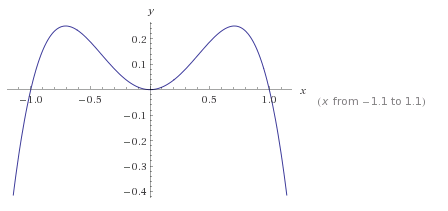
\includegraphics[scale=0.5]{TEqualToZeroAndVEqualToOne}

\vspace{3mm}

For $t=1$ and $\nu=1$, we obtain the following equation and graph:

\vspace{3mm}

$u(x,t)=\frac{1}{2} \bigg[(x+1)^2(1-(x+1)^2)+(x-1)^2(1-(x-1)^2)\bigg]$

\vspace{3mm}

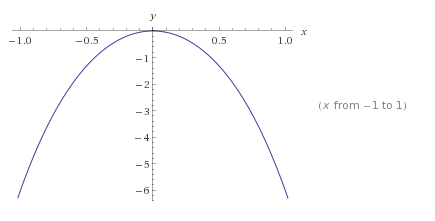
\includegraphics[scale=0.5]{TAndVEqual1}

\vspace{3mm}

For $t=2$ and $\nu=1$, we obtain the following equation and graph:

\vspace{3mm}

$u(x,t)=\frac{1}{2} \bigg[(x+2)^2(1-(x+2)^2)+(x-2)^2(1-(x-2)^2)\bigg]$

\vspace{3mm}

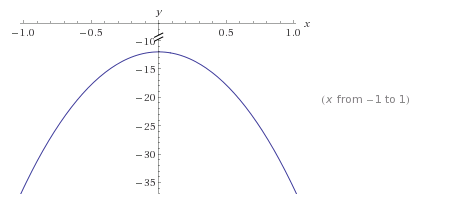
\includegraphics[scale=0.5]{TEqualToTwoAndVEqualToOne}

\vspace{3mm}

\pagebreak

\vspace*{-40mm}

For $t=3$ and $\nu=1$, we obtain the following equation and graph:

\vspace{3mm}

$u(x,t)=\frac{1}{2} \bigg[(x+3)^2(1-(x+3)^2)+(x-3)^2(1-(x-3)^2)\bigg]$

\vspace{3mm}

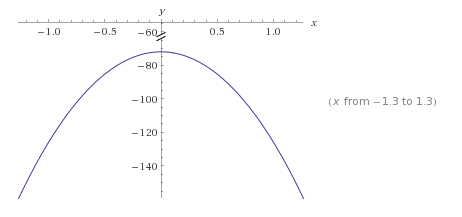
\includegraphics[scale=0.5]{TEqualToThreeAndVEqualTo1}

\vspace{3mm}

For $t=0$ and $\nu=2$, we obtain the following equation and graph:

\vspace{3mm}

$u(x,t)=\frac{1}{2} \bigg[x^2(1-x^2)+x^2(1-x^2)\bigg]$

\vspace{3mm}

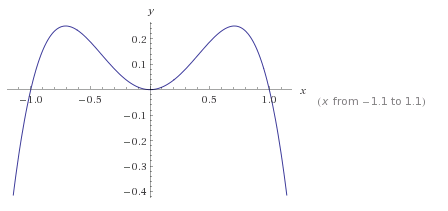
\includegraphics[scale=0.5]{TEqualToZeroAndVEqualToOne}

\vspace{3mm}

For $t=1$ and $\nu=2$, we obtain the following equation and graph:

\vspace{3mm}

$u(x,t)=\frac{1}{2} \bigg[(x+2)^2(1-(x+2)^2)+(x-2)^2(1-(x-2)^2)\bigg]$

\vspace{3mm}

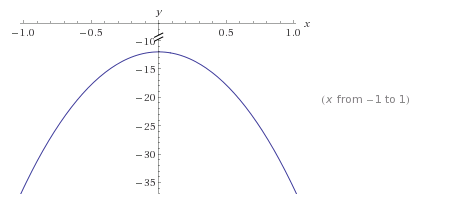
\includegraphics[scale=0.5]{TEqualToTwoAndVEqualToOne}

\vspace{3mm}

\pagebreak

\vspace*{-40mm}

For $t=2$ and $\nu=2$, we obtain the following equation and graph:

\vspace{3mm}

$u(x,t)=\frac{1}{2} \bigg[(x+4)^2(1-(x+4)^2)+(x-4)^2(1-(x-4)^2)\bigg]$

\vspace{3mm}

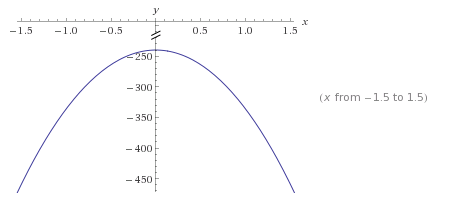
\includegraphics[scale=0.5]{TEqualToTwoAndVEqualToTwo}

\vspace{3mm}

For $t=2$ and $\nu=3$, we obtain the following equation and graph:

\vspace{3mm}

$u(x,t)=\frac{1}{2} \bigg[(x+6)^2(1-(x+6)^2)+(x-6)^2(1-(x-6)^2)\bigg]$

\vspace{3mm}

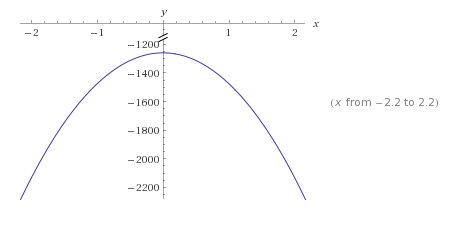
\includegraphics[scale=0.5]{TEqualToThreeAndVEqualToTwo}

\vspace{3mm}

As the values of $t$ increase in both the cases where $\nu=1$ and $\nu=2$, the wave propagates more and more to the left.

\end{flushleft}

\begin{flushleft}

3)The function $u(x,t)=\frac{1}{2} \bigg[(x+\nu t)^2(1-(x+\nu t)^2)+(x-\nu t)^2(1-(x-\nu t)^2)\bigg]$ is not a solution to the initial value problem for the wave equation according to \textit{d\textsc{\char13}Alembert\textsc{\char13}s theorem} because the piecewise function does not satisfy the condition of having both of its derivatives being continuous over all of $\mathbb{R}$. We should not be using this theorem because our piecewise function does not fully satisfy the hypothesis of \textit{d\textsc{\char13}Alembert\textsc{\char13}s theorem}.

\end{flushleft}

\vspace{3mm}

\begin{flushleft}

4) As the hint in the assignment says: just replace the $t$ with a $\nu$ and we obtain $\nu(x,t)=\frac{1}{2} \bigg[(x+\nu t)^2(1-(x+\nu t)^2)+(x-\nu t)^2(1-(x-\nu t)^2)\bigg]$.

\end{flushleft}

\vspace{3mm}

\begin{flushleft}

5) Before time equal to zero i.e. the initial point in time, there is no physical force in our physical setting. 

\end{flushleft}

\begin{flushleft}

6) We wish to translate $\frac{\partial^2 w}{\partial t^2}=\nu^2\frac{\partial^2 w}{\partial x^2}$ into $\frac{-1}{4\nu^2}f\bigg(\frac{\xi+\eta}{2}, \frac{\xi-\eta}{2\nu}\bigg)$. To begin, define $\xi=x-\nu t$ and $\eta=x+\nu t$. Then, we have the following:

\pagebreak

\vspace*{-40mm}

\begin{center}

$\frac{\partial w}{\partial t}=-\nu \bigg(\frac{\partial w}{\partial \xi}\bigg) \bigg(\frac{\partial \xi}{\partial t}\bigg) + \nu \bigg(\frac{\partial w}{\partial \zeta}\bigg) \bigg(\frac{\partial \zeta}{\partial t}\bigg)$

\vspace{3mm}

We then take a second derivative with respect to $t$ and have

\vspace{3mm}

$\frac{\partial}{\partial t}\bigg(\frac{\partial w}{\partial t}\bigg)= \frac{\partial}{\partial t} \bigg[-\nu \frac{\partial w}{\partial \xi} + \nu \frac{\partial w}{\partial \zeta}\bigg]$

\vspace{3mm}

Next, we take derivatives with respect to $\xi$ and $\zeta$ to end up with:

\vspace{3mm}

$\frac{\partial^2 w}{\partial t^2}= \frac{\partial }{\partial \xi} \bigg[-\nu \frac{\partial w}{\partial \xi} + \nu \frac{\partial w}{\partial \zeta}\bigg] \frac{\partial \xi}{\partial t}+ \frac{\partial}{\partial \zeta} \bigg[\nu \frac{\partial w}{\partial \xi}+\nu \frac{\partial w}{\partial \zeta}\bigg] \frac{\partial \zeta}{\partial t}$

\vspace{3mm}

$\frac{\partial^2 w}{\partial t^2}=\nu^2  \frac{\partial^2 w }{\partial \xi^2} -\nu \frac{\partial^2 w}{\partial \xi \partial \zeta} - \nu \frac{\partial ^2 w}{\partial \zeta \partial \xi} + \nu^2 \frac{\partial^2 w}{\partial \zeta^2}$

\vspace{3mm}

After combing common partial derivatives, we have:

\vspace{3mm}

$\frac{\partial^2 w}{\partial t^2}=\nu^2 \frac{\partial^2 w }{\partial \xi^2} -2\nu^2 \frac{\partial^2 w}{\partial \xi \partial \zeta} + \nu^2 \frac{\partial^2 w}{\partial \zeta^2}$

\vspace{3mm}

After using $\frac{\partial^2 w}{\partial t^2}=\nu^2\frac{\partial^2 w}{\partial x^2}$ and moving terms around, we end up with:

\vspace{3mm}

$\nu^2 \frac{\partial^2 w }{\partial \xi^2} -2\nu^2 \frac{\partial^2 w}{\partial \xi \partial \zeta} + \nu^2 \frac{\partial^2 w}{\partial \zeta^2}=\nu^2 \frac{\partial^2 w }{\partial \xi^2} +2\nu^2 \frac{\partial^2 w}{\partial \xi \partial \zeta} + \nu^2 \frac{\partial^2 w}{\partial \zeta^2}+f\bigg(\frac{\xi+\eta}{2}, \frac{\xi-\eta}{2\nu}\bigg)$

\vspace{3mm}

Combining like terms results in:

\vspace{3mm}

$-4\nu^2 \frac{\partial^2 w}{\partial \xi \partial \zeta}=f\bigg(\frac{\xi+\eta}{2}, \frac{\xi-\eta}{2\nu}\bigg)$

\vspace{3mm}

Dividing through by the $4\nu^2$ terms leaves us with

\vspace{3mm}

$\frac{\partial^2 w}{\partial \xi \partial \zeta}=\frac{1}{4\nu^2}f\bigg(\frac{\xi+\eta}{2}, \frac{\xi-\eta}{2\nu}\bigg)$, as desired.

\end{center}

\end{flushleft}

\begin{flushleft}

7) The function $w$ is defined by $w(\xi, \zeta)=\frac{1}{4\nu^2} \int\limits_{\vphantom{b}\zeta}^{\infty}\int\limits_{-\infty}^{\xi} f\bigg(\frac{\xi'+\zeta'}{2}, \frac{\xi'-\zeta'}{2\nu}\bigg) \mathrm{d}\xi' \mathrm{d}\zeta'$ where $\xi'$ and $\zeta'$ are dummy variables. To verify that this function satisfies the wave equation, which we defined in \#6 to be $\frac{\partial ^2 w}{\partial \xi \partial \zeta}=\frac{-1}{4\nu^2}f\bigg(\frac{\xi+\eta}{2}, \frac{\xi-\eta}{2\nu}\bigg)$, we must take the derivative with respect to $\xi$ using the limit definition of a derivate:

\vspace{3mm}

\begin{center}

$w=\frac{1}{4\nu^2} \lim_{\substack{a\to\infty \\ b\to-\infty}} \int\limits_{\vphantom{b}\zeta}^{\infty}\int\limits_{-\infty}^{\xi} f\bigg(\frac{\xi'+\zeta'}{2}, \frac{\xi'-\zeta'}{2\nu}\bigg) \mathrm{d}\xi' \mathrm{d}\zeta'$

\vspace{3mm}

$w=\frac{-1}{4\nu^2} \lim_{\substack{a\to\infty \\ b\to-\infty}} \int\limits_{\vphantom{b}\zeta}^{\infty}\int\limits_{-\infty}^{\xi} f\bigg(\frac{\xi'+\zeta'}{2}, \frac{\xi'-\zeta'}{2\nu}\bigg) \mathrm{d}\xi' \mathrm{d}\zeta'$

\pagebreak

\vspace*{-40mm}

Then, when you take the derivatives with a and b plugged into the above formula, the terms with a and b are constant so the derivatives are $0$. So the limit doesn't depend on a and b. This results in:

\vspace{3mm}

$\frac{\partial w}{\partial \xi}=\frac{-1}{4\nu^2} \lim_{b\to-\infty} \int\limits_{\vphantom{b}\zeta}^{\infty}f\bigg(\frac{\xi'+\zeta'}{2}, \frac{\xi'-\zeta'}{2\nu}\bigg) \mathrm{d}\xi'$

\vspace{3mm}

and

\vspace{3mm}

$\frac{\partial^2 w}{\partial \zeta \partial \xi}=\frac{-1}{4\nu^2}f\bigg(\frac{\xi'+\zeta'}{2}, \frac{\xi'-\zeta'}{2\nu}\bigg)$

\end{center}

\end{flushleft}

\begin{flushleft}

8) If one draws the region in the $\xi$, $\zeta$ plane described by the limits of integration, the result will be a pair of intersecting lines that form a "X". Then, if one rotates these lines 45\degree clockwise, then the area we wish to integrate, if we suppose that we are in the $x$, $t$ plane, would be the space between the $x-axis$ and and the triangle formed by the intersecting lines. Next, to obtain the outer limits of integration, note that $f(x,t)=0 \forall t < 0$. This means that when we integrate the area described above, we are not concerned with any area where $t < 0$ and only want to start integrating at the point where $t=0$, and since both lines extend infinitely in the $t$ direction, we want to be able to integrate up to any arbitrary $t$ value. Hence, the outer bounds go from $0$ up to $t$.

\vspace{3mm}

To obtain the lower bounds of integration, make note of the following equations:

\begin{center}

$\xi=x+\nu t$, $\zeta=x-\nu t$, $\xi'=x'+\nu t$, and $\zeta'=x'-\nu t$

\vspace{3mm}

Then, we have the following:

$x+\nu t=x'+\nu t$

\vspace{1mm}

$\nu'=x+\nu t-\nu t'$

\vspace{1mm}

$x'=x+\nu(t-t')$

\vspace{3mm}

and

\vspace{3mm}

$x-\nu t=x'-\nu t$

\vspace{1mm}

$x'=x-\nu t+\nu t'$

\vspace{1mm}

$x'=x-\nu(t-t')$

\vspace{4mm}

Then, to go from the $\frac{1}{4\nu^2}$ to $\frac{1}{2\nu}$, note that we have the following equations:

\vspace{3mm}

$x=\frac{1}{2} \xi + \frac{1}{2} \zeta$ and $f=\frac{1}{2\nu} \xi - \frac{1}{2\nu} \zeta$

\vspace{3mm}

Then, if we take some derivatives and plug them into the Jacobian matrix, we have:

\vspace{3mm}

$ \begin{pmatrix}
  \frac{\partial x}{\partial \xi} & \frac{\partial x}{\partial \zeta} \\
  
  		&\\
  
\frac{\partial t}{\partial \xi} & \frac{\partial t}{\partial \zeta}\\
 \end{pmatrix}=\begin{pmatrix}
  \frac{1}{2} & \frac{1}{2} \\
  
  		&\\
  
\frac{-1}{2\nu} & \frac{1}{2\nu}\\
 \end{pmatrix}$
 
\pagebreak

\vspace*{-40mm}
 
 Then, take the determinant and we get:
 
 \vspace{3mm}
 
$\frac{1}{4\nu} +  \frac{1}{4\nu}=\frac{2}{4\nu}=\frac{1}{4\nu}$

\end{center}

\end{flushleft}

\begin{flushleft}

9) $w(x,t)$ satisfies the inhomogeneous equation because we used the equation, changed variables, took some derivatives, and then changed variables back to the ones we started with. For the initial conditions, we have:

\begin{center}

$w(x,0)=\frac{1}{2\nu} \int\limits_{\vphantom{b}0}^{0}\int\limits_{x-\nu(t-t')}^{x+\nu(t-t')} f(x',t') \mathrm{d}x' \mathrm{d}t'$

\vspace{3mm}

$w(x,0)=\frac{1}{2\nu} \int\limits_{\vphantom{b}0}^{0}0$

\vspace{3mm}

$w(x,0)=\frac{1}{2\nu}(0)$

\vspace{5mm}

and 

\vspace{5mm}

$w(x,0)=\frac{1}{2\nu} \int\limits_{\vphantom{b}0}^{0}\int\limits_{x-\nu(t-t')}^{x+\nu(t-t')} f(x',t') \mathrm{d}x' \mathrm{d}t'$

\vspace{3mm}

taking the partial derivative with respect to $t$ gives:

$\frac{\partial w}{\partial t} (x,t) \frac{1}{2\nu} \bigg[f'(x',t') \Big|_0^t \int\limits_{x-\nu(t-t')}^{x+\nu(t-t')} f(x',t') \mathrm{d}x' \mathrm{d}t' \bigg]$

\vspace{3mm}

Next, plus in $t=0$ according to our initial conditions, resulting in:

\vspace{3mm}

$\frac{\partial w}{\partial t} (x,t) \frac{1}{2\nu} [0] \bigg[\int\limits_{x-\nu(t-t')}^{x+\nu(t-t')} f(x',t') \mathrm{d}x' \mathrm{d}t' \bigg]$

\vspace{3mm}

Which, simplifies to:

\vspace{3mm}

$\frac{\partial w}{\partial t}=0$

\end{center}

\vspace{3mm}

Thus, putting together what we have done, we arrive at:

\begin{center}

$w(x,t)=\frac{1}{2\nu} \int\limits_{\vphantom{b}0}^{t}\int\limits_{x-\nu(t-t')}^{x+\nu(t-t')} f(x',t') \mathrm{d}x' \mathrm{d}t'$

\end{center}

\end{flushleft}

\begin{flushleft}

10)Using the work we obtained for the $\nu$-problem and the $w$-problem and supposing that the solution to the inhomogeneous wave equation is of the form:

\begin{center}

$u(x,t)=\nu(x,t)+w(x,t)$

\end{center}

the solution to the inhomogeneous wave equation is:

\pagebreak

\vspace*{-40mm}

\begin{center}

$u(x,t)=\frac{1}{2} \bigg[(x+\nu t)^2(1-(x+\nu t)^2)+(x-\nu t)^2(1-(x-\nu t)^2)\bigg]+\frac{1}{2\nu} \int\limits_{\vphantom{b}0}^{t}\int\limits_{x-\nu(t-t')}^{x+\nu(t-t')} f(x',t') \mathrm{d}x' \mathrm{d}t'$

\end{center}

\end{flushleft}

\end{document}